\chapter{Semantic Web Technologies}


\begin{figure}[htbp]
    \centering
    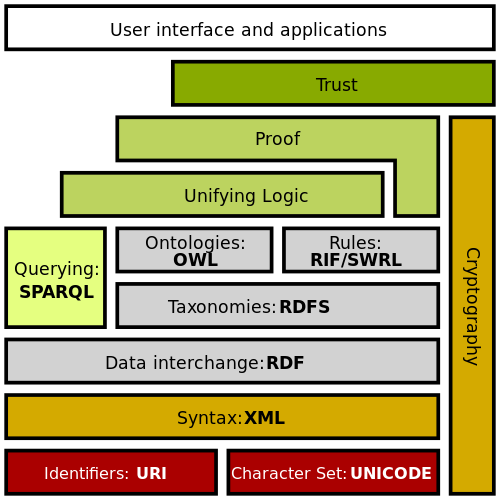
\includegraphics[width=0.5\textwidth]{fig/Semantic_web_stack.svg.png}
    \caption{An overview of semantic web stack with core technologies\cite{sem_web_stack}.}
    \label{fig:sem_web_stack}
\end{figure}

Semantic web extends the existing \emph{web of documents} with the ability 
to \emph{link} different documents and \emph{embed knowledge} in the document
to transform it into a \emph{web of data}. It is perceived by Tim Beners-Lee in 
2001\cite{bernerslee2001semantic} to be integrated into the existing architecture 
of World Wide Web. Embedding \emph{knowledge} into documents enables machines to
interpret the \emph{meaning} of the document and interoperate with each other on 
a more complex level.

Semantic web stack enables one to start building a \emph{web of data} using 
the core technologies shown in Figure~\ref{fig:sem_web_stack}. 
However, this is provided that the data already exists in RDF compliant format.
Existing data on the web in non-RDF format must, therefore, be transformed 
into RDF data enable transition to a \emph{web of data}. This work 
focuses on transforming non-RDF to RDF data, thus the RDF format will be elaborated 
in detail. 



\section{RDF}
Resource Definition Framework \cite{rdf_concepts} is a framework for representing data on the Web.
It portrays the data as a directed graph with the resources as nodes in the graph and the
edges as the relationship between the different resources.
Figure~\ref{fig:rdf_triple_ex} shows an example of an RDF triple statement describing
the information “John has an apple”.
The triple statement consists of the subject \textit{John}, the predicate \textit{has}
and the object \textit{apple}.

\begin{figure}[htbp]
    \centering
    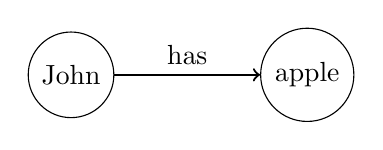
\begin{tikzpicture}[node distance={30mm}, main/.style = {draw, circle}]

        \node[main] (subject) {John};
        \node[main] (object) [right of=subject] {apple};

        \draw[->, thick] (subject) -- node[midway, above, sloped] {has} (object);

    \end{tikzpicture}
    \caption{An RDF triple representing the information “John has an apple”.}

    \label{fig:rdf_triple_ex}
\end{figure}


By composing these simple triple statements into a set of RDF triples, it yields us an RDF graph.
In Figure~\ref{fig:rdf_graph_ex}, 4 triple statements are composed together to form a
simple RDF graph describing \textit{John} and \textit{Mary} having the same \textit{apple}.
It might not be evident from the simple figures, about the advantages of
RDF graphs. Data representation in a graph model allows machines to follow the
\textit{links} between the resources, and discover more unknown
data in the linked knowledge graph. Link following is possible due to the nodes in
the triples being classified as one of the 3 different term types.

\begin{figure}[htbp]
\centering
\begin{tikzpicture}[node distance={45mm}, main/.style = {draw, circle}]

\node[main] (subject) {John};
\node[main] (subject_2) [below of=subject] {Mary};
\node[main] (object) [right of=subject] {apple};
\node[main] (apple_object_colour) [above right of=object] {red};
\node[main] (apple_object_ripe) [below right of=object, text width=15mm] {Malus domestica};
\node [cloud, draw,cloud puffs=10,cloud puff arc=120, aspect=2, inner ysep=1em]
(colour_kg) [below right of=apple_object_colour] {colours KG};

\draw[->, thick] (subject) -- node[midway, above, sloped] {has} (object);
\draw[->, thick] (subject_2) -- node[midway, above, sloped] {has} (object);
\draw[->, thick] (apple_object_colour) -- (colour_kg);
\draw[->, thick] (object) -- node[midway, above, sloped] {has colour} (apple_object_colour);
\draw[->, thick] (object) -- node[midway, above, sloped] {scientific name} (apple_object_ripe);
\end{tikzpicture}
\caption{A simple RDF graph where the same “apple” is shared by both John and Mary.}
\label{fig:rdf_graph_ex}
\end{figure}

\subsection{Term types}
Resources are classified into 3 different term types; IRI (Internationalized Resource Identifier),
literals and blank nodes. IRI is a string identifier unique in the global scope to
represent a resource. It is usually in the form of a web address, however, it can
also be in other forms so long as it conforms to the syntax defined in
RFC 3987~\footnote{RFC 3987: \url{https://www.ietf.org/rfc/rfc3987.txt}}.
IRI can represent a relationship, a concept or an object. Therefore, it could be
used in the \textit{subject}, the \textit{predicate} and the \textit{object} components of
an RDF triple.

Literals term type is used to represent a value such as strings, numbers, boolean and dates.
To ensure that the machines know the type of the data being read, we could
explicitly specify the type of the data with a datatype IRI. Moreover, the
language in which the data is written, could also be explicitly stated with
a language tag.

Lastly, we have the term type blank nodes. Blank nodes identify resources
in the local scope (i.e. to a local file or an RDF store). Since it is used to
identify resources in nodes, blank nodes are only applicable as the \textit{subject}
and the \textit{object} components of an RDF triple.


\subsection{TURTLE syntax}
The aforementioned term types are defined for abstract RDF syntax. For a concrete syntax to write
RDF triples, we would focus on the TURTLE (Terse RDF Triple Language)~\cite{turtle_syntax}
syntax in this work. A simple triple statement is a sequence of
\textit{subject, predicate, object} terms, ending in a '.'.
To reduce the repetition of writing the same subject and predicate combination with
different objects, TURTLE allows the use of ',' to separate the different objects.
Additionally, one could also use ';' to separate the different predicates and objects sharing the
same subject. 


\begin{lstlisting}[label={lst:same_subject}, 
    caption={Usage of ';' where triples share the same subject.}]
<http://example.org/apple>  <http://example.org/hasColor> "red";
                            <http://example.org/scientificName> "Malus domestica".
\end{lstlisting}

\begin{lstlisting}[label={lst:different_object}, 
    caption={Usage of ',' where triples differs only in the objects.}]
<http://example.org/apple>  <http://example.org/scientificName> "Malus pumila", 
                                                                "Malus domestica".
\end{lstlisting}


IRIs are written between the angle brackets like \lstinline{<http://example.org/#John>}.
Since blank nodes are locally scoped version of IRIs, the same syntax to write IRIs is also used.
TURTLE syntax allows us to define \textit{prefixes} at the head of the TURTLE file.
Users could then use prefixes, to write RDF triples in a more compact form. For example,
\lstinline{<http://example.org/#John>} could be shortened to
\lstinline{<#John>} using the relative \textit{@base} path.

\begin{lstlisting}[caption=Prefixes in TURTLE syntax.]
    @base <http://example.org/> . # default base IRI
    @prefix rdf: <http://www.w3.org/1999/02/22-rdf-syntax-ns#> .
    @prefix rdfs: <http://www.w3.org/2000/01/rdf-schema#> .
    @prefix foaf: <http://xmlns.com/foaf/0.1/> .
    @prefix rel: <http://www.perceive.net/schemas/relationship/> . 
    ... 
\end{lstlisting}

Literals are written between the double quote '"'. It has a default datatype of 
a string. One could also \textit{cast} the literal value to a specific datatype 
by appending '\textasciicircum{} \textasciicircum{} $[$IRI of the datatype$]$'. For example, 
"12" is cast to an integer in \lstinline{"12"^^xsd:integer}. Language of the literal value 
could also be specified using \textit{@} similarly to datatype casting. 
